
%(BEGIN_QUESTION)
% Copyright 2006, Tony R. Kuphaldt, released under the Creative Commons Attribution License (v 1.0)
% This means you may do almost anything with this work of mine, so long as you give me proper credit

Calculate the following voltage drops in this circuit assuming a thermocouple tip temperature of 718$^{o}$ F, perfect calibration of all other instruments in the loop (Temp. range = 500 to 1000$^{o}$ F; current range = 4 to 20 mA), and a DC power supply voltage of exactly 28 volts:

$$\includegraphics[width=15.5cm]{i00393x01.eps}$$

\begin{itemize}
\item{} Voltage between terminals TB64-8 and TB64-9 =
\vskip 5pt
\item{} Voltage between terminals TB64-10 and TB64-11 =
\vskip 5pt
\item{} Voltage between terminals TB27-15 and TB27-16 =
\end{itemize}

\vskip 10pt

Also, determine where you could connect a {\it loop calibrator} device to substitute for the transmitter, and what mode the calibrator should be set to in order to control the loop current.

\vskip 20pt \vbox{\hrule \hbox{\strut \vrule{} {\bf Suggestions for Socratic discussion} \vrule} \hrule}

\begin{itemize}
\item{} Demonstrate how to {\it estimate} numerical answers for this problem without using a calculator.
\item{} Discuss the options we have for thermocouple tip styles, and how this particular thermocouple's tip characteristics compare with others.
\item{} Explain what ``downscale burnout'' means and why this transmitter configuration might be significant.
\item{} What exactly is a ``paperless'' chart recorder?
\item{} What would happen in this system if the local indicator (TI-14) were to electrically fail open?
\end{itemize}

\underbar{file i00393}
%(END_QUESTION)





%(BEGIN_ANSWER)

\begin{itemize}
\item{} Voltage between terminals TB64-8 and TB64-9 = 22.512 volts
\vskip 5pt
\item{} Voltage between terminals TB64-10 and TB64-11 = 2.744 volts
\vskip 5pt
\item{} Voltage between terminals TB27-15 and TB27-16 = 25.256 volts
\end{itemize}

\vskip 10pt

Hint: if you are having difficulty analyzing this circuit, try re-drawing it in schematic form (all current-carrying components in a straight line to show their series connections).

%(END_ANSWER)





%(BEGIN_NOTES)

A loop calibrator could be set to ``Simulate'' mode and connected where the transmitter used to connect (disconnecting the transmitter first).  Alternatively, the loop could be opened and the calibrator used to ``Source'' current directly to the 250 ohm resistor.








\filbreak \vskip 20pt \vbox{\hrule \hbox{\strut \vrule{} {\bf Virtual Troubleshooting} \vrule} \hrule}

\noindent
{\bf Predicting the effect of a given fault:} present each of the following faults to the students, one at a time, having them comment on all the effects each fault would produce.

\begin{itemize}
\item{} 
\item{} 
\item{} 
\end{itemize}


\vskip 10pt


\noindent
{\bf Identifying possible/impossible faults:} present symptoms to the students and then have them determine whether or not a series of suggested faults could account for all the symptoms, explaining {\it why} or {\it why not} for each proposed fault:

\begin{itemize}
\item{} Symptom: {\it Suppose TIR-14 registers below 500 degrees F}
\item{} TY-14a resistor failed open -- {\bf Yes}
\item{} TY-14a resistor failed shorted -- {\bf No}
\item{} TY-14b resistor failed open -- {\bf No}
\item{} TY-14b resistor failed shorted -- {\bf Yes}
\item{} TE-14 failed open -- {\bf Yes}
\item{} TE-14 failed shorted -- {\bf Yes}
\item{} Cable CBL9 failed open -- {\bf Yes}
\item{} Cable CBL9 failed shorted -- {\bf No}
\item{} Cable CBL22 failed open -- {\bf Yes}
\item{} Cable CBL22 failed shorted -- {\bf No}
\end{itemize}


\vskip 10pt


\noindent
{\bf Determining the utility of given diagnostic tests:} present symptoms to the students and then propose the following diagnostic tests one by one.  Students rate the value of each test, determining whether or not it would give useful information (i.e. tell us something we don't already know).  Students determine what different results for each test would indicate about the fault, if anything:

\begin{itemize}
\item{} Symptom: {\it }
\item{}  -- {\bf Yes/No}
\item{}  -- {\bf Yes/No}
\end{itemize}


\vskip 10pt


\noindent
{\bf Diagnosing a fault based on given symptoms:} imagine the ??? fails ??? in this system (don't reveal the fault to students!).  Present the operator's observation(s) to the students, have them consider possible faults and diagnostic strategies, and then tell them the results of tests they propose based on the following symptoms, until they have properly identified the nature and location of the fault:

\begin{itemize}
\item{} Operator observation: {\it }
\item{} 
\item{} 
\end{itemize}
%INDEX% Basics, loop-powered transmitter: voltage drop calculations
%INDEX% Documentation, loop diagram

%(END_NOTES)


